\section{Broadcast Channel}
A broadcast channel is a communication channel with one sender and two or more receivers. It is shown in the figure \ref{fig:BC}. Here, the basic problem is finding the set of simultaneously achievable rates for communication in a broadcast channel. Let us consider some examples of broadcast channels.
%
\begin{figure}[h]
    \centering
    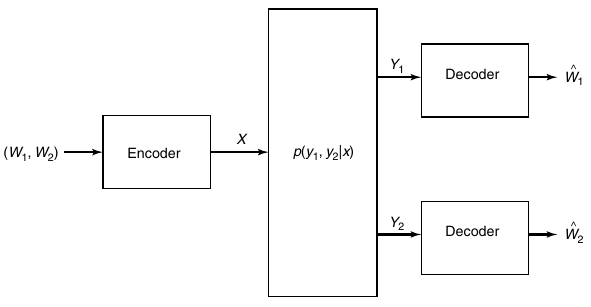
\includegraphics[scale=0.5]{Diagrams/BC.png}
    \caption{A Broadcast Channel.}
    \label{fig:BC}
\end{figure}
%

\subsection{Some examples}
\subsubsection*{TV Station}
The TV (or radio) station is one of the simplest and most common examples of broadcast channels. This channel is degenerate because the station wants to send the same information to multiple users who are tuned in. However, the better receiver (\textit{e.g.} HDTV) will receive extra information than the worst receiver (\textit{e.g.} B\&W TV). Therefore we need to rearrange the information in that way. It is schematically shown in the figure \ref{fig:TVBC}.
%
\begin{figure}[h]
    \centering
    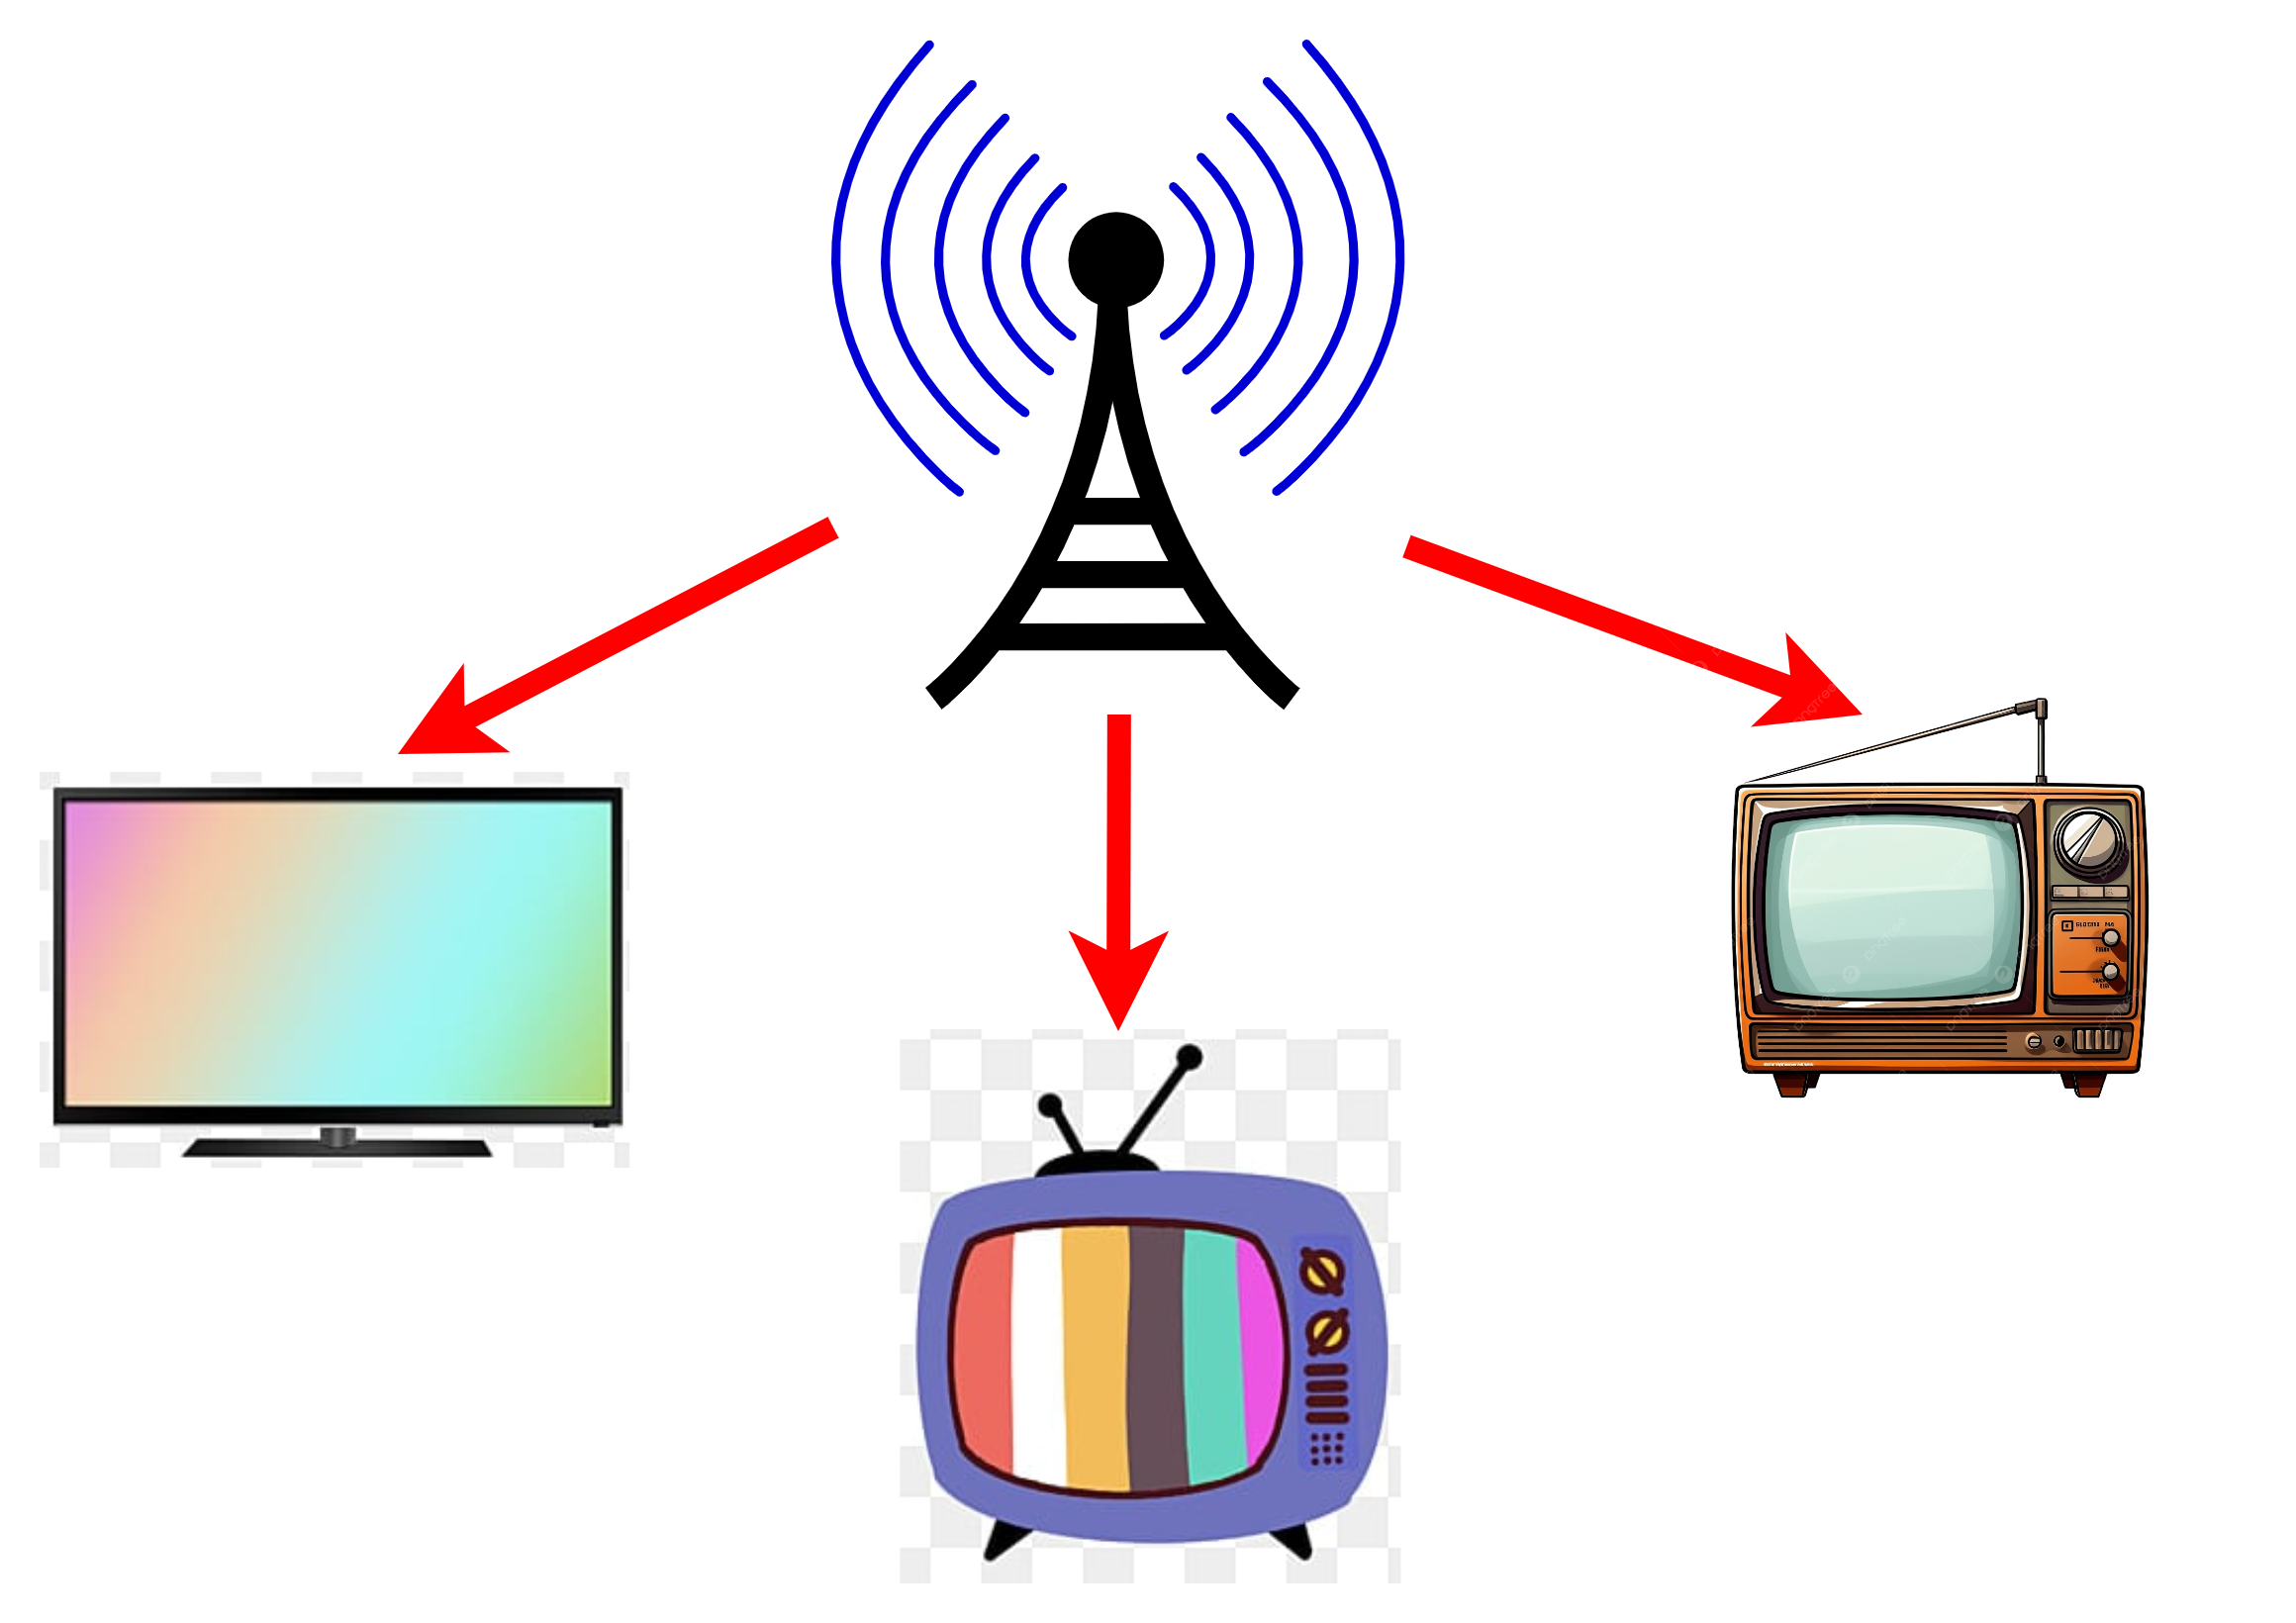
\includegraphics[width=0.4\linewidth]{Presentation Diagrams/TVBC.png}
    \caption{A broadcast TV Channel consists of four components: one station and three receivers.}
    \label{fig:TVBC}
\end{figure}
%

%%%%%%%%%%%%%%%%%%%%%%%%%%%%%%%%%%%%%%%%%%%%%%%%%%%%%%%%%%%%%%%%%%%%%%%%%%%
\subsection{ Some Definitions and Theorem}

\begin{tcolorbox}[boxrule=0pt,frame hidden,sharp corners,enhanced, opacityback=0, borderline west={2pt}{0pt}{red}]
\begin{defn} \textbf{(A broadcast channel)} A broadcast channel consists of an input alphabet $\mathcal{X}$ and two output alphabets, $\mathcal{Y}_1$ and $\mathcal{Y}_2$, and a probability transition function $p(y_1,y_2|x)$. The broadcast channel will be said to be memoryless if
%
\begin{eqnarray}
p(y_1^n|y_2^n|x^n) = \prod_{i=1}^n p(y_{1i}, y_{2i}|x_i)   
\end{eqnarray}
%
\end{defn}
\end{tcolorbox}
%
Now, let us define some important concepts in the case of a broadcast channel. But it is similar to the multiple-access channel. 
%
\begin{tcolorbox}[boxrule=0pt,frame hidden,sharp corners,enhanced, opacityback=0, borderline west={2pt}{0pt}{red}]
\begin{defn} \textbf{(A $((2^{nR_1},2^{nR_2}),n)$ code)} A $((2^{nR_1},2^{nR_2}),n)$ code for the broadcast channel consists of two sets of integers $\mathcal{W}_1 = \{1,2,...,2^{nR_1} \}$ and $\mathcal{W}_2 = \{1,2,...,2^{nR_2} \}$, called the message sets, an encoding function,
%
\begin{eqnarray}
    X: (\mathcal{W}_1 \times \mathcal{W}_2) \rightarrow \mathcal{X}^n,
\end{eqnarray}
%
and two decoders,
%
\begin{eqnarray}
    g_1: \mathcal{Y}_1^n \rightarrow \mathcal{W}_1.
\end{eqnarray}
%
and
%
\begin{eqnarray}
    g_2: \mathcal{Y}_2^n \rightarrow \mathcal{W}_2.
\end{eqnarray}
%
\end{defn}
\end{tcolorbox}
%
As shown in the diagram \ref{fig:BC}, there are one sender and two receivers for this channel. Let us define the average probability of error.
%
\begin{tcolorbox}[boxrule=0pt,frame hidden,sharp corners,enhanced, opacityback=0, borderline west={2pt}{0pt}{red}]
\begin{defn} \textbf{(Average Probability of error)} The average probability of error for the $((2^{nR_1},2^{nR_2}),n)$ code is given by
%
\begin{eqnarray}
    P_e^{(n)} = P(g_1(Y^n_1) \neq W_1 \text{ or } g_2(Y^n_2) \neq W_2)),
\end{eqnarray}
%
where $(W_1, W_2)$ are assumed to be uniformly distributed over $2^{nR_1}\times 2^{nR_2}$.
\end{defn}
\end{tcolorbox}
%
If common information needs to be sent to both receivers, we need to define a different code as well as different rates.
%
%
\begin{tcolorbox}[boxrule=0pt,frame hidden,sharp corners,enhanced, opacityback=0, borderline west={2pt}{0pt}{red}]
\begin{defn} \textbf{(A $((2^{nR_0}, 2^{nR_1},2^{nR_2}),n)$ code)} A $((2^{nR_1},2^{nR_2}),n)$ code for a broadcast channel with common information consists of three sets of integers $\mathcal{W}_0 = \{1,2,...,2^{nR_0} \}$, $\mathcal{W}_1 = \{1,2,...,2^{nR_1} \}$, and $\mathcal{W}_2 = \{1,2,...,2^{nR_2} \}$, called the message sets, an encoder,
%
\begin{eqnarray}
    X: (\mathcal{W}_0 \times \mathcal{W}_1 \times \mathcal{W}_2) \rightarrow \mathcal{X}^n,
\end{eqnarray}
%
and two decoders,
%
\begin{eqnarray}
    g_1: \mathcal{Y}_1^n \rightarrow \mathcal{W}_0 \times \mathcal{W}_1.
\end{eqnarray}
%
and
%
\begin{eqnarray}
    g_2: \mathcal{Y}_2^n \rightarrow \mathcal{W}_0 \times \mathcal{W}_2.
\end{eqnarray}
%
\end{defn}
\end{tcolorbox}
%
Let us assume that the $(W_0, W_1, W_2)$ distribution is uniform. Therefore,
%
\begin{tcolorbox}[boxrule=0pt,frame hidden,sharp corners,enhanced, opacityback=0, borderline west={2pt}{0pt}{red}]
\begin{defn} \textbf{(Average Probability of error)} The average probability of error for the $((2^{nR_0}, 2^{nR_1},2^{nR_2}),n)$ code is given by
%
\begin{eqnarray}
    P_e^{(n)} = P(g_1(Y^n_1) \neq (W_0, W_1) \text{ or } g_2(Z^n) \neq (W_1, W_2)),
\end{eqnarray}
%
\end{defn}
\end{tcolorbox}
%
Now, we can define the rate triple as follows:
%
\begin{tcolorbox}[boxrule=0pt,frame hidden,sharp corners,enhanced, opacityback=0, borderline west={2pt}{0pt}{red}]
\begin{defn} \textbf{(A rate pair $(R_0, R_1, R_2)$)} A rate pair $(R_0, R_1, R_2)$ is said to be achievable for the broadcast channel with common information if there exists a sequence of $((2^{nR_0}, 2^{nR_1},2^{nR_2}),n)$ codes with $P_e^{(n)}\rightarrow 0$.
\end{defn}
\end{tcolorbox}
%
Finally, we would define the capacity region for the broadcast channel.
%
\begin{tcolorbox}[boxrule=0pt,frame hidden,sharp corners,enhanced, opacityback=0, borderline west={2pt}{0pt}{red}]
\begin{defn} \textbf{(The capacity region)} The capacity region of the broadcast is the closure of the set of achievable rates.
\end{defn}
\end{tcolorbox}
%
The error for receiver $Y_1^n$ depends inky on the conditional marginal distributions $p(x^n, y_1^n)$ and not on the joint distribution $p(x^n, y_1^n, y_2^n)$. Therefore,
%
\begin{tcolorbox}[boxrule=0pt,frame hidden,sharp corners,enhanced, opacityback=0, borderline west={2pt}{0pt}{blue}]
\begin{thm} 
The capacity region of a broadcast channel depends only on the conditional marginal distributions $p(y_1|x)$ and $p(y_2|x)$.
%
\end{thm}
\end{tcolorbox}
%
%%%%%%%%%%%%%%%%%%%%%%%%%%%%%%%%%%%%%%%%%%%%%%%%%%%%%%%%%%%%%%%%%%%%%%%%
\subsection{Degraded Broadcast Channels}
Let us define the degraded broadcast channels.
%
\begin{tcolorbox}[boxrule=0pt,frame hidden,sharp corners,enhanced, opacityback=0, borderline west={2pt}{0pt}{red}]
\begin{defn} \textbf{(Physically degraded broadcast channel)} A broadcast channel is said to be physically degraded if $p(y_1,y_2|x) = p(y_1|x)p(y_2|y_1)$.
\end{defn}
\end{tcolorbox}
%
%
\begin{tcolorbox}[boxrule=0pt,frame hidden,sharp corners,enhanced, opacityback=0, borderline west={2pt}{0pt}{red}]
\begin{defn} \textbf{(Stochastically degraded broadcast channel)} A broadcast channel is said to be stochastically degraded if its conditional marginal distributions are the same as that of a physically degraded broadcast channel; that is, if there exists a distribution $p'(y_2|y_1)$ such that 
%
\begin{eqnarray}
    p(y_2|x) = \sum_{y_1} p(y_1|x)p'(y_2|y_1).
\end{eqnarray}
%
\end{defn}
\end{tcolorbox}
%
The capacity of the stochastically degraded broadcast channel is identical to that of the corresponding physically degraded channel as the broadcast channel's capacity is only dependent on the conditional marginals.

%%%%%%%%%%%%%%%%%%%%%%%%%%%%%%%%%%%%%%%%%%%%%%%%%%%
\subsection{Capacity Region for the Degraded Broadcast Channel}
Let us consider sending independent information through a degraded broadcast channel at the rate $R_1$ to $Y_1$ and rate $R_2$ to $Y_2$.
%
\begin{tcolorbox}[boxrule=0pt,frame hidden,sharp corners,enhanced, opacityback=0, borderline west={2pt}{0pt}{blue}]
\begin{thm} 
The capacity region for sending independent information over the degraded broadcast channel $X \rightarrow Y_1 \rightarrow Y_2$ is the convex hull of the closure of all $(R_1, R_2)$ satisfying
%
\begin{eqnarray}
    R_2 \leq I(U;Y_2), \\
    R_1 \leq I(X; Y_1|U),
\end{eqnarray}
%
for some joint distribution $p(u)p(x|u)p(y_1,y_2|x)$, where the auxiliary random varibale $U$ has cardinality bounded by $\abs{U} \leq \min\{\abs{\mathcal{X}}, \abs{\mathcal{Y}_1}, \abs{\mathcal{Y}_2} \}$.
\end{thm}
\end{tcolorbox}
%
%
\begin{tcolorbox}[boxrule=0pt,frame hidden,sharp corners,enhanced, opacityback=0, borderline west={2pt}{0pt}{blue}]
\begin{thm} 
If the rate pair $(R_1, R_2)$ is achievable for a degraded broadcast channel, the rate triple $(R_0, R_1, R_2-R_0)$ is achievable for the channel with common information, provided that $R_0 < R_2$.
\end{thm}
\end{tcolorbox}
%
%%%%%%%%%%%%%%%%%%%%%%%%%%%%%%%%%%%%%%%%%%%

\subsection{Some Examples}
%
\subsubsection{A pair of Binary Symmetric Channel}
Let us consider a pair of binary symmetric channels with error probability $p_1$ and $p_2$. This pair of channels construct a broadcast channel, as shown in the figure \ref{fig:bsbc}. We assume that $p_1 < p_2< \frac{1}{2}$. \\
%
\begin{figure}[h]
\centering
\begin{minipage}{.35\textwidth}
  \centering
  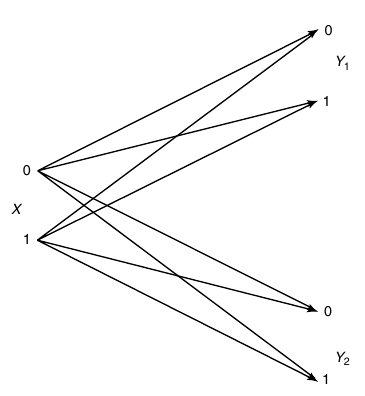
\includegraphics[scale=0.4]{Diagrams/BSBC.png}
  \captionof{figure}{Binary Symmetric Broadcast Channel}
  \label{fig:bsbc}
\end{minipage}%
\hspace{2 em}
\begin{minipage}{.55\textwidth}
  \centering
  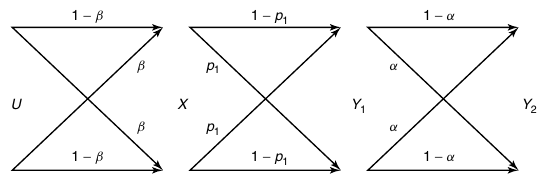
\includegraphics[scale=0.5]{Diagrams/BSDBC.png}
  \captionof{figure}{Physically degraded binary symmetric broadcast channel}
  \label{fig:bsdbc}
\end{minipage}
\end{figure}
%
This channel can be expressed as a cascade of a binary symmetric channel with parameter $p_1$ and the crossover probability of the new channel $\alpha$. Then, for the overall crossover probability of the cascade:
%
\begin{enumerate}
    \item With probability \( p_1 \), the first channel introduces an error.

    \begin{itemize}
        \item If there’s an error in the first channel (with probability \( p_1 \)), then the probability that the second channel doesn’t introduce an error is \( (1 - \alpha) \).

        \item Thus, the contribution to the overall error probability from this case is \( p_1 (1 - \alpha) \).
    \end{itemize}

    \item With probability \( (1 - p_1) \), the first channel does not introduce an error.

    \begin{itemize}
        \item If there’s no error in the first channel (with probability \( 1 - p_1 \)), then the probability that the second channel introduces an error is \( \alpha \).

        \item Thus, the contribution to the overall error probability from this case is \( (1 - p_1) \alpha \).
    \end{itemize}
\end{enumerate}
 %
Adding these contributions gives the overall probability of an error after both channels:
%
\begin{eqnarray}
    && p_1 (1 - \alpha) + (1 - p_1) \alpha = p_2 \nonumber\\
    \implies && \alpha = \frac{p_2-p_1}{1-2p_1}
\end{eqnarray}
%
Now, let us consider the auxiliary random variable in the definition of the capacity region. From the theorem, the cardinality of $U$ is binary from the bound. As shown in figure \ref{fig:bsdbc}, symmetry allows us to link $U$ and $X$ via a second binary symmetric channel with parameter $\beta$. \\
The rates in the capacity region may now be computed. Symmetry makes it evident that the uniform distribution on $\{0, 1\}$ is the distribution on U that optimizes the rates, such that
%
\begin{eqnarray}
    I(U;Y_2) = H(Y_2)-H(Y_2|U) = 1-H(\beta * p_2),
\end{eqnarray}
%
where $\beta * p_2 = \beta(1-p_2)+(1-\beta)p_2$. Similarly,
%
\begin{eqnarray}
    I(X;Y_1|U) &=& H(Y_1|U)-H(Y_1|X,U) \nonumber\\
    &=& H(Y_1|U)-H(Y_1|X) \nonumber\\
    &=& H(\beta * p_1)-H(p_1),
\end{eqnarray}
%
where $\beta * p_1 = \beta(1-p_1)+(1-\beta)p_1$. Now, by plotting these points, we can obtain the capacity region. Let us analyze the corner points:
%
\begin{enumerate}
    \item \textbf{When $\beta = 0$:} Maximum information will be transfer to $Y_2$ as
    %
    \begin{eqnarray*}
        R_2 = 1-H(p_2) \text{ and } R_1 = 0.
    \end{eqnarray*}

    \item \textbf{When $\beta = \frac{1}{2}$:} Maximum information will be transfer to $Y_1$ as
    %
    \begin{eqnarray*}
        R_1 = 1-H(p_1) \text{ and } R_2 = 0.
    \end{eqnarray*}
    %
    \textit{i.e.}, no information will be transferred to $Y_2$.
\end{enumerate}
%
This leads to the plot, as shown in the figure.
%
\begin{figure}[h]
    \centering
    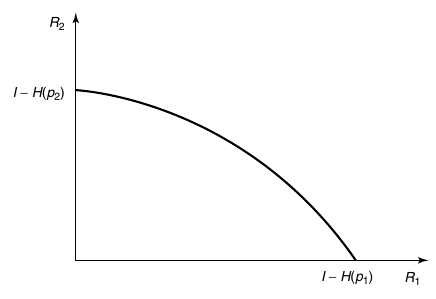
\includegraphics[scale= 0.5]{Diagrams/CRBSBC.png}
    \caption{Capacity region of binary symmetric broadcast channel}
    \label{fig:CRBSBC}
\end{figure}
%
%%%%%%%%%%%%%%%%%%%%%%
\subsubsection{Gaussian Broadcast Channel}
The Gaussian broadcast channel is shown in figure \ref{fig:GBC}. Here, one output is a degraded version of the other output. Therefore from the figure, we can write
%
\begin{eqnarray}
    Y_1 &=& X+Z_1 \\
    Y_2 &=& X+Z_2 = Y_1+Z_2',
\end{eqnarray}
%
where $Z_1 \sim \mathcal{N}(0, N_1)$ and $Z_2' \sim \mathcal{N}(0, N_2-N_1)$. As discussed in the earlier section, the result can be extended in this case too. Therefore, the capacity region of this channel is given by
%
\begin{eqnarray}
    R_1 &<& C\lrfb{\frac{\alpha P}{N_1}} \\
    R_2 &<& C\lrfb{\frac{(1-\alpha) P}{\alpha P+N_2}},
\end{eqnarray}
%
where $\alpha$ may be arbitrarily chosen $(0 \leq \alpha \leq 1)$.
%
\begin{figure}[h]
    \centering
    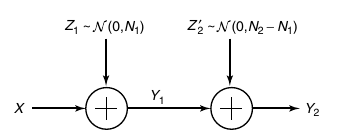
\includegraphics[scale=0.6]{Diagrams/GBC.png}
    \caption{Gaussian Broadcast Channel}
    \label{fig:GBC}
\end{figure}